\documentclass[journal,transmag]{IEEEtran}

% ..........................................................................
% Packages, configuration settings, and macro definitions.

\usepackage[pdftex]{graphicx}
\graphicspath{figures}
\DeclareGraphicsExtensions{.pdf,.jpeg,.png}

\usepackage[pdftex,rgb,dvipsnames,svgnames,hyperref,table]{xcolor}

\usepackage[pdftex,breaklinks=true,colorlinks=true,
	bookmarks=false,pdfhighlight=/O,
	urlcolor=DarkBlue,citecolor=DarkRed,linkcolor=DarkBlue]{hyperref}

\usepackage[cmex10]{amsmath}
\interdisplaylinepenalty=2500

\usepackage{amssymb}
\usepackage{amsfonts}
\usepackage{multicol}
\usepackage{multirow}
\usepackage{enumitem}
\usepackage{accsupp}
\usepackage{array}
\usepackage[caption=false,font=footnotesize]{subfig}
\usepackage{booktabs}
\usepackage{xspace}
\usepackage{soul}
\usepackage{url}
\usepackage{hyphenat}
\usepackage[english]{babel}

% Correct bad hyphenation here
\hyphenation{op-tical net-works semi-conduc-tor ana-ly-tics}

\usepackage{pdfcomment}
\newcommand{\comment}[3]{\pdfmarkupcomment[markup=Highlight,color=yellow,author={#2}]{#1}{#3}}

\usepackage{tabularx}
% ..........................................................................
% Body.

\begin{document}

\markboth{IEEE Transactions on Biomedical Engineering}{Standards for whole-cell modeling}

\title{Toward standards for tomorrow's whole-cell models}

\author{
	\IEEEauthorblockN{
		Dagmar Waltemath\IEEEauthorrefmark{1},
		Falk Schreiber\IEEEauthorrefmark{2,3}, 
		Jonathan R. Karr\IEEEauthorrefmark{4}, 
%        Michael Hucka\IEEEauthorrefmark{5},
%        Chris J. Myers\IEEEauthorrefmark{6},
%        Frank T. Bergmann\IEEEauthorrefmark{5,7,8},\\
%        Vijayalakshmi Chelliah\IEEEauthorrefmark{9},
%        Marcus Krantz\IEEEauthorrefmark{10},
%        Wolfram Liebermeister\IEEEauthorrefmark{11},
%        Pedro Mendes\IEEEauthorrefmark{12--15},
%        Pinar Pir\IEEEauthorrefmark{16},
        Begum Alaybeyoglu\IEEEauthorrefmark{17},
        Rafael S. Costa\IEEEauthorrefmark{18},\\
        Muhammad Haseeb\IEEEauthorrefmark{19},
        Vincent Knight-Schrijver\IEEEauthorrefmark{16},
        Sucheendra K. Palaniappan\IEEEauthorrefmark{20},
        Martin Scharm\IEEEauthorrefmark{1},\\
        Kieran Smallbone\IEEEauthorrefmark{21} and
        Markus Wolfien\IEEEauthorrefmark{1}
%        2015 Whole-Cell Modeling Summer School Consortium\IEEEauthorrefmark{5} 
        }
	
	\IEEEauthorblockA{\IEEEauthorrefmark{1}Department of Systems Biology and Bioinformatics, University of Rostock}
	\IEEEauthorblockA{\IEEEauthorrefmark{2}Clayton School of Information Technology, Monash University}
    \IEEEauthorblockA{\IEEEauthorrefmark{3}Institute of Computer Science, Martin Luther University Halle-Wittenberg}    
	\IEEEauthorblockA{\IEEEauthorrefmark{4}Department of Genetics \& Genomic Sciences, Icahn School of Medicine at Mount Sinai} 
        %New York, NY 10029 USA\\Email: \href{mailto:karr@mssm.edu}{karr@mssm.edu}
%    \IEEEauthorblockA{\IEEEauthorrefmark{5}Department of Computing and Mathematical Sciences, California Institute of Technology} 
        %1200 East California Boulevard, Pasadena, CA 91125, USA
%    \IEEEauthorblockA{\IEEEauthorrefmark{6}Department of Electrical and Computer Engineering, University of Utah} 
        %Salt Lake City, Utah 84112, USA
%    \IEEEauthorblockA{\IEEEauthorrefmark{7}BioQuant, University of Heidelberg} 
        %Heidelberg , Germany
%    \IEEEauthorblockA{\IEEEauthorrefmark{8}Centre for Organismal Studies, University of Heidelberg} 
%    \IEEEauthorblockA{\IEEEauthorrefmark{9}European Molecular Biology Laboratory, European Bioinformatics Institute} 
        %Wellcome Trust Genome Campus, Hinxton, Cambridge CB10 1SD, UK viji@ebi.ac.uk.
%    \IEEEauthorblockA{\IEEEauthorrefmark{10}Department of Biology, Humboldt University of Berlin} 
        %Berlin, Germany
%    \IEEEauthorblockA{\IEEEauthorrefmark{11}Institute of Biochemistry, Charit\'e Medical University of Berlin} 
        %10117 Berlin, Germany
%    \IEEEauthorblockA{\IEEEauthorrefmark{12}Manchester Institute of Biotechnology, University of Manchester} 
%    \IEEEauthorblockA{\IEEEauthorrefmark{13}School of Computer Science, University of Manchester}     
%    \IEEEauthorblockA{\IEEEauthorrefmark{14}Center for Quantitative Medicine, University of Connecticut Health Center}
%    \IEEEauthorblockA{\IEEEauthorrefmark{15}Department of Cell Biology, University of Connecticut Health Center}
        %131 Princess Street, Manchester, M1 7DN, UK. pedro.mendes@manchester.ac.uk
        %Farmington, Connecticut, USA
%    \IEEEauthorblockA{\IEEEauthorrefmark{16}Babraham Institute}
    \IEEEauthorblockA{\IEEEauthorrefmark{17}Department of Chemical Engineering, Bo\v{g}azi\c{c}i University}
    \IEEEauthorblockA{\IEEEauthorrefmark{18}Instituto Superior T\'ecnico, University of Lisbon}
    \IEEEauthorblockA{\IEEEauthorrefmark{19}Department of Bioinformatics, Mohammad Ali Jinnah University}
    \IEEEauthorblockA{\IEEEauthorrefmark{20}Rennes - Bretagne Atlantique Research Centre, Institute for Research in Computer Science and Automation}
    \IEEEauthorblockA{\IEEEauthorrefmark{21}Manchester Centre for Integrative Systems Biology, University of Manchester}    
    %\IEEEauthorblockA{\IEEEauthorrefmark{5}Membership of the 2015 Whole-Cell Modeling Summer School Consortium is listed in Table~SI}
    %
	\thanks{Corresponding author email: \href{mailto:dagmar.waltemath@uni-rostock.de}{dagmar.waltemath@uni-rostock.de}}
}

\IEEEtitleabstractindextext{
	\begin{abstract}
	Whole-cell models are a promising tool for biological research, bioengineering, and medicine. 
	However, significant work remains to achieve fully complete and accurate whole-cell models, including developing a strong theoretical understanding of multi-algorithm modeling and an efficient general-purpose simulators.
	We organized the 2015 Whole-Cell Modeling Summer School to evaluate the need for new whole-cell modeling standards by assessing the ability of SBML to represent a recently published whole-cell model, as well as to teach whole-cell modeling.
    We believe that three SBML extensions are needed to support transparent, reproducible whole-cell modeling: support for multi-algorithm model composition, support for particle-based representation, and support for template reactions. In addition, we believe that new user-friendly graphical model editors and parallelized simulators are needed to efficiently build and simulate whole-cell models.
	Together, we believe that these new standards and software tools will enable researchers to realize the full potential of whole-cell modeling.
	\end{abstract}
	
	% Note that keywords are not normally used for peer review papers.
	\begin{IEEEkeywords}
	Whole-cell modeling, Systems biology, Computational biology, Mathematical modeling, Simulation, Standards, Education
	\end{IEEEkeywords}
}

\maketitle
\IEEEdisplaynontitleabstractindextext
\IEEEpeerreviewmaketitle

\section{Introduction}

% The very first letter is a 2 line initial drop letter followed by the rest of the first word in caps.
% 
% form to use if the first word consists of a single letter:
% \IEEEPARstart{A}{demo} file is ....
% 
% form to use if you need the single drop letter followed by normal text (unknown if ever used by IEEE):
% \IEEEPARstart{A}{}demo file is ....
% 
% Some journals put the first two words in caps:
% \IEEEPARstart{T}{his demo} file is ....
% 
% Here we have the typical use of a "T" for an initial drop letter and "HIS" in caps to complete the first word.
% is a report of the VW Whole-cell Summer School held in Rostock during April 2015.

\IEEEPARstart{O}{ver} the past twenty years, computational modeling has become an essential and powerful tool for biological research, bioengineering, and medicine to analyze high-throughput molecular measurements and understand the molecular details of complex biological systems. 
Computational modeling has already been used to identify new metabolic genes~\cite{Reed2006}, add metabolic pathways to bacteria~\cite{Lee2009}, and identify potential new antimicrobial drug targets~\cite{Lee2012}. 
Computational models also have the potential to enable bioengineers to design new microorganisms for industrial applications such as chemical synthesis, biofuel production, and waste decontamination, as well as to enable clinicians to design personalized medical therapies tailored to each individual patient's unique genome. 
Realizing this potential requires more comprehensive and accurate computational models which are capable of predicting cellular behavior from genotype, as well as standardized methods for exchanging models, simulation experiments, and model visualizations~\cite{Macklin2014,Karr2015,hucka2015promoting,Klipp07}.

Recently, researchers at Stanford University developed the first whole-cell model of the gram-positive bacterium \textit{Mycoplasma genitalium}~\cite{Karr2012}. 
The model represents the life cycle of a single Mycoplasma cell including the copy number dynamics of each metabolite, RNA, and protein species and accounts for every known gene function. 
The model is comprised of 28 sub-models, each of which is implemented using different mathematical representations including ordinary differential equations (\emph{ODE}s), flux balance analysis (\emph{FBA}), and Boolean rules (\emph{BR}s), and trained using different experimental data. 

The \textit{M. genitalium} whole-cell model was implemented in MATLAB, is available open-source under the MIT license, and is extensively documented. 
This has enabled other researchers to use the model for their own research and enabled educators to use the model to teach systems biology. 

However, the \textit{M. genitalium} model software is not general-purpose. Consequently, significant domain expertise is required to use the model or construct new whole-cell models. 
New whole-cell modeling standards and simulation tools are needed to enable more researchers to develop and use their own whole-cell models. 
Such standards would accelerate the whole-cell modeling field. They would enable researchers to develop models more quickly, more deeply explore model predictions, and more rigorously evaluate models. Furthermore, they would enable researchers to contribute whole-cell models to model repositories such as BioModels~\cite{li2010biomodels} which in turn, would make models more searchable, retrievable, reusable, and comparable.

Several systems biology standards have already been developed by the COmputational Modeling in BIology NEtwork (\emph{COMBINE})~\cite{le2011meeting} including the Systems Biology Markup Language (\emph{SBML})~\cite{hucka2003}, the Cell Markup Language (\emph{CellML})~\cite{hedley_2001b}, the Simulation Experiment Description Markup Language (\emph{SED-ML})~\cite{sedml2011}, and the Systems Biology Graphical Notation (\emph{SBGN})~\cite{LeNovereHMMSS09}. SBML and CellML are standard languages for describing mathematical models including ODE, logical, and FBA models. Both have been used to build thousands of models of various intracellular pathways. SED-ML is a standard language for describing computational experiments. SED-ML enables computational scientists to reproduce simulations by describing simulation setups in detail, including the simulation algorithm and every parameter value. SBGN is a standard which provides three language for describing visual representations of models. However, none of these standards have been used to construct, simulate, or visualize models as large as the \textit{M. genitalium} whole-cell model.

We organized the 2015 Whole-Cell Modeling Summer School to evaluate the need for new standards for whole-cell modeling, as well as to train students in whole-cell modeling. The course included two introductory lectures on whole-cell modeling and the existing systems biology standards and featured three days of hands-on active learning in which students were divided into small groups, each of which was responsible for evaluating the ability of SBML to represent one or more of the \textit{M. genitalium} sub-models.

Here, we propose three SBML extensions to support whole-cell modeling and report the educational outcomes of the summer school. 
First, we summarize the summer school. 
Second, we describe our progress toward encoding the \textit{M. genitalium} whole-cell model using SBML. 
Lastly, we describe the SBML, SED-ML, and SBGN expansions needed to encode whole-cell models.

\section{The 2015 Whole-Cell Modeling Summer School}
One of the main goals of the summer school was to teach students how to build models and encode models using COMBINE standards through encoding the \textit{M. genitalium} model using only standard representation formats and open-source simulation software.

\subsection{Organization}
We began the school with two lectures to introduce the students to whole-cell modeling and the existing systems biology standards. Jonathan Karr from the Icahn School of Medicine at Mount Sinai, USA presented an overview of whole-cell and multi-algorithm modeling. Michael Hucka from the California Institute of Technology, USA presented an overview of the SBML, SED-ML, and SBGN standards; open-source software tools which support those standards; and the COMBINE initiative. In addition to the introductory lectures, we organized three discussions on three common SBML encoding problems: particle-based state representation, random number generation, and sub-model integration. 

The majority of the school was dedicated to hands-on active learning sessions in which students learned about whole-cell modeling and the COMBINE standards by trying to encode parts of the \textit{M. genitalium} whole-cell model using SBML. Students were divided into ten groups of four to five students, eight of which were tasked with trying to recode sub-models of the \textit{M. genitalium} model, one of which was tasked with developing a scheme to integrate all of the sub-models into a single model, and one of which was responsible for helping the other eight groups document and visualize their models. Table~SI lists the ten groups and all of the students and tutors. 

We concluded each day with brief progress reports from each group. The progress reports facilitated discussion on common standards encoding challenges, provided groups opportunities to get feedback from each other, and helped the integration group plan the assembly of the integrated model.

To facilitate student networking, we also organized a poster session, as well as several evening social activities.

\subsection{Educational outcomes}
\comment{Following the school, we surveyed the students to assess the educational outcome of the course.}{Karr}{What do the surveys actually say?}
Most students reported that they gained deeper knowledge of whole-cell modeling, more appreciation for the importance of reproducibility, and increased understanding of the SBML, SED-ML, and SBGN standards.
Many students also reported that they learned about open-source modeling software tools which are applicable for their graduate research.

In addition, many of the students reported that the course helped them network with other systems biologists. 
In particular, several students reported that the course introduced them to other systems biology opportunities including open postdoctoral positions and the 2016 Whole-Cell Modeling Summer School (\href{http://www.wholecell.org/school-2016}{http://www.wholecell.org/school-2016}).

\subsection{Lessons learned for organizing summer schools}
We learned several valuable lessons about how to best organize summer schools.
First, we found that summer schools must have clear learning objectives.
Second, we found that students greatly enjoy hands-on active learning rather than didactic lectures. 
Furthermore, we found that a high teacher to student ratio and a flexible schedule are necessary to successfully run open-ended project-based courses.
Third, we found that students should be divided into multidisciplinary teams. 
This enables students to learn from other scientists with alternative perspectives from other fields and builds strong teams that are well-equipped to solve difficult problems.
In the case of this summer school, it also enabled us to quickly assess potential expansions to SBML to support whole-cell models from multiple perspectives, ensuring that the expanded standards will meet the needs of modelers, software developers, and model curators.
Fourth, we found that social activities greatly enhance summer schools by encouraging informal networking interactions among students.
Lastly, we found that summer schools must have generous financial support. This enables organizers to accept students irrespective of their funding status. In turn, this enables the course to include a broader range of students than would otherwise be possible.


\section{Progress toward an SBML-encoded whole-cell model}
In addition to training young computational systems biology researchers, the second goal of the course was to recode the \textit{M. genitalium} whole-cell model using SBML. To achieve this goal, eight groups of four

Specifically, eight of the ten groups were responsible for encoding one or more sub-models. The ninth group focused on developing a standards-compliant scheme for integrating SBML-encoded sub-models into a single model. This group was responsible for defining the sub-model interfaces and developing a SED-ML scheme to simulate the entire model.
The tenth group focused on helping the other groups.
The group members advised with the modeling, developed a generic annotation scheme, helped visualize the sub-models using SBGN, and assisted in documentation.
Each group was led by an experienced tutor.

The groups pursued various strategies to encode the sub-models using SBML. Several of the groups encoded sub-models by first reading the sub-model documentation, second drawing pathway maps using software tools such as Cell Designer~\cite{funahashi2008celldesigner} and VANTED~\cite{Rohn2012}, and then writing scripts to automatically generate SBML representations from their maps. Other groups used modeling software tools such as COPASI~\cite{Mendes2009} and BioUML~\cite{Kolpakov2006} to encode sub-models based on their documentation. A third set of groups encoded sub-models by converting the original MATLAB code to SBML. These groups then automatically generated SBGN maps from their SBML to better understand their sub-models.

iBioSim

the course produced preliminary SBML and SBGN-ML versions of each of the \textit{M. genitalium} whole-cell model sub-models.
Since the course, the project groups have continued to meet online to complete the encoding and testing of their sub-models.
We plan to complete the encoding and integration of the advanced sub-models into a single model in a two-days satellite meeting to the COMBINE in October 2015. 
%into a single model within the next few months.

The sub-models and integrated model will be encoded using SBML, and simulatable with open-source simulation software tools such as COPASI, BioUML, and iBioSim~\cite{Madsen2012}.
The sub-models and integrated model will be available open-source at \url{http://github.com/whole-cell-tutors/wholecell} and the BioModels database.
We believe the sub-models and integrated model will be a valuable community resource which will enable other scientists to develop, expand, and apply whole-cell models to their own research.

We are organizing a second meeting in conjunction with the 2015 COMBINE meeting in Salt Lake City, USA to finish recoding and testing the sub-models.

\section{Limitations of SBML, SED-ML, and SBGN for whole-cell modeling}
Prior to the summer school, SBML, SED-ML, and SBGN had never been used to represent similarly large or complex models. 
Consequently, the summer school revealed several limitations of SBML, SBGN, and the existing simulation software for large models.
First, no general-purpose simulation software supports multi-algorithm models such as the \textit{M. genitalium} whole-cell model. 
Second, SBML does not support sparse representations of large, combinatorial state spaces. Consequently, every state space must be enumerated. For the case of the \textit{M. genitalium} model, this means that the chromosome state space must be enumerated, resulting in millions of state variables and unmanageably large XML files.
Third, the existing SBML simulation tools have limited support for arrays. Consequently, matrix operations that were efficiently implemented and executed in MATLAB, must be enumerated, resulting in verbose, opaque SBML files and inefficient simulations.
Fourth, the existing SBML simulation tools have limited support random number generation which is required to encode many of the sub-models. Consequently, many of the sub-models must be recast as Gillespie algorithm simulations to be supported by SBML.

The summer school also revealed  limitations of SBGN for whole-cell models. 
First, whole-cell modeling requires SBGN maps which contain a mixture of Process Description, Entity Relationship, and Activity Flow nodes. Currently, SBGN maps can only contain one of these three types of nodes.
Second, whole-cell modeling demands improved support for automatic layout of large maps. The layout algorithms available are mostly not tailored to the specific networks occurring within a whole-cell model. 
Third, to reduce the complexity it would be helpful to provide generic forms of other entities in the same map, an issue already discussed within the SBGN community.

Most importantly, the summer school facilitated discussions among modelers, software tools developers, and model curators about how to best overcome these limitations.

However, neither language supports several of the features needed for whole-cell modeling including large, sparsely occupied state spaces and multi-algorithm simulations. 

 SBGN can be used to visualize large models. However, additional features are needed to compactly visualize large models including support for mixed diagrams and generic reactions. whole-cell modeling requires hybrid SBGN maps which contain a mixture of the three SBGN languages. Currently, SBGN maps can only contain glyphs from one of the three languages. Second, whole-cell modeling demands improved support for automatic layout of large maps. The layout algorithms available are mostly not tailored to the specific networks occurring within a whole-cell model.  Third, to reduce the complexity it would be helpful to provide generic reactions in a map, such that the overall number of reactions shown could be significantly reduced.
Taken together, further work is needed to expand the capabilities of the current systems biology standard languages to support whole-cell modeling.

These courses should provide students opportunities to learn about techniques for integrating multiple sub-models and resolving conflicts including state locking, adaptive time-stepping, controllers and semaphores; how to identify the parameters of large models including numerical optimization, distributed optimization, and model reduction; and how to test models using unit testing and continuous integration. 

\section{Conclusion}

The 2015 Whole-Cell Modeling Summer School successfully trained 45 young scientists in whole-cell multi-algorithm modeling and the existing systems biology modeling standards. Additional summer schools and courses are needed to provide students deeper theoretical training in dynamical modeling, multi-algorithm modeling, and parameter estimation, as well as practical training in model construction including data curation, model building, model testing, and model analysis. 

The summer school also made significant strides toward recoding the \textit{M. genitalium} whole-cell model using SBML for simulation by COMBINE software. However, significant work remains to expand SBML to support whole-cell models, recode the \textit{M. genitalium} model using SMBL, and develop general-purpose simulation software programs which are capable of efficiently simulating multi-algorithm models. Since the Rostock meeting, some of the working groups have continued to recode their sub-models and several of the students and tutors plan to participate in a second working meeting at the 2015 COMBINE Forum at the University of Utah in Salt Lake City, USA. We hope to publish some of the recoded sub-models to the BioModels database.

Ultimately, in order to achieve an integrated, SBML-encoded whole-cell model, SBML must be expanded to support multi-algorithm modeling and efficiently encode large, combinatorial state spaces using a particle-based representations. In addition, higher-level SBML constructs are needed to compactly represent template reactions, new graphical editors are needed to enable modelers to efficiently construct large models, new parallelized simulators are needed to quick simulate large models, and new parameter estimation tools are needed to help researchers automatically identify parameter values from large-scale experimental data.

We believe that whole-cell modeling has the potential to be an important tool for biological discovery, bioengineering, and medicine.
Achieving this potential requires improved standards for transparently communicating whole-cell models, as well as general-purpose simulation software for reproducibly simulating whole-cell models.
In turn, this requires expanding the whole-cell modeling field including training young researchers in whole-cell modeling.

\section*{Acknowledgments}
The course was supported by a grant from the Volkswagen Foundation to DW and FS. JRK was supported by a James S. McDonnell Foundation Postdoctoral Fellowship Award in Studying Complex Systems.

\ifCLASSOPTIONcaptionsoff
  \newpage
\fi

\bibliographystyle{IEEEtran}
\bibliography{IEEEabrv,report}

% biography section
% 
% If you have an EPS/PDF photo (graphicx package needed) extra braces are needed around the contents of the optional argument to biography to prevent
% the LaTeX parser from getting confused when it sees the complicated \includegraphics command within an optional argument. (You could create
% your own custom macro containing the \includegraphics command to make things simpler here.)

\begin{IEEEbiography}[{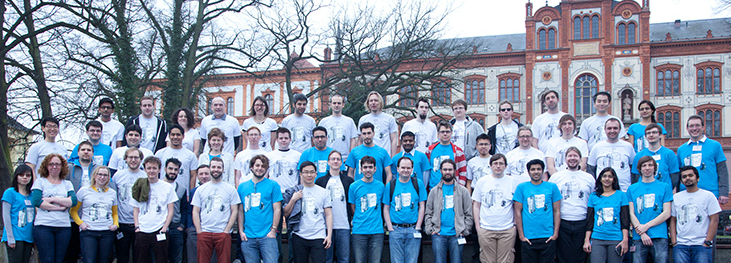
\includegraphics[width=3.48in,keepaspectratio]{photos/group.jpg}}]{}
~\\
~\\
~\\
~\\
~\\
~\\
~\\
~\\
~\\
~\\
~\\
\textbf{2015 Whole-Cell Modeling Summer School} included the 56 researchers listed in Table~SI.
\end{IEEEbiography}


% You can push biographies down or up by placing a \vfill before or after them. The appropriate
% use of \vfill depends on what kind of text is on the last page and whether or not the columns are being equalized.

\vfill

% Can be used to pull up biographies so that the bottom of the last one is flush with the other column.
%\enlargethispage{-5in}

% ..........................................................................
% End.

\clearpage
\setcounter{table}{0}
\renewcommand{\thetable}{S\Roman{table}}

\begin{table*}[ht!]
\caption{2015 Whole-Cell Modeling Summer School Consortium members.}
\begin{tabularx}{\textwidth}{l||l||X}\hline
\bfseries Group        & \bfseries Participant            & \bfseries Affiliation\\\hline\hline
Cytokinesis            & Naveen Kumar Aranganathan        & University Paris-Sud, France\\
                       & Daniel Alejandro Priego Espinosa & National Autonomous University of Mexico, Mexico\\
                       & Ilya Kiselev                     & Siberian Branch of the Russian Academy of Sciences Novosibirsk, Russia\\
                       & Wolfram Liebermeister            & Charit\'e Medical University of Berlin, Germany\\
                       & Yan Zhu                          & Monash University, Australia\\\hline
DNA repair             & Arne Bittig                      & University of Rostock, Germany\\
                       & Vijayalakshmi Chelliah           & European Bioinformatics Institute, UK\\
                       & Audald Lloret-Vilas              & European Bioinformatics Institute, UK\\
                       & Mahesh Sharma                    & National Institute of Pharmaceutical Education and Research, India\\
                       & Namrata Tomar                    & Friedrich-Alexander University of Erlangen-N\"urnberg, Germany\\\hline
Metabolism             & Kambiz Baghalian                 & University of Oxford, UK\\
                       & Frank T. Bergmann                & California Institute of Technology, USA\\
                       & Rafeal Sousa Costa               & University of Lisbon, Portugal\\
                       & Matthias K\"onig                 & Charit\'e Medical University of Berlin, Germany\\
                       & Kieran Smallbone                 & University of Manchester, UK\\
                       & Milenko Tokic                    & Swiss Federal Institute of Technology in Lausanne, Switzerland\\\hline
Protein                & Begum Alaybeyoglu                & Bo\v{g}azi\c{c}i University, Turkey\\
                       & Matteo Cantarelli                & OpenWorm, UK\\
                       & Yin Hoon Chew                    & University of Edinburgh, UK\\
                       & Marcus Krantz                    & Humboldt University of Berlin, Germany\\
                       & Daewon Lee                       & KAIST, South Korea\\\hline
Replication            & Vincent Knight-Schrijver         & Babraham Institute, UK\\
                       & Je-Hoon Song                     & KAIST, South Korea\\
                       & Jannis Uhlendorf                 & Humboldt University of Berlin, Germany\\
                       & Dagmar Waltemath                 & University of Rostock, Germany\\
                       & James Yurkovich                  & University of California, San Diego, USA\\
                       & Anna Zhukova                     & University of Bordeaux, France\\\hline
Replication initiation & Harold Gomez                     & Boston University, USA\\
                       & Jens Hahn                        & Humboldt University of Berlin, Germany\\
                       & Michael Hucka                    & California Institute of Technology, USA\\
                       & Nikita Mandrik                   & Siberian Branch of the Russian Academy of Sciences Novosibirsk, Russia\\
                       & Martin Scharm                    & University of Rostock, Germany\\
                       & Florian Wendland                 & University of Rostock, Germany\\\hline
RNA                    & Tuure Hameri                     & Swiss Federal Institute of Technology in Lausanne, Switzerland\\
                       & Jesse Kyle Medley                & University of Washington, USA\\
                       & Sucheendra Kumar Palaniappan     & Institute for Research in Computer Science and Automation, France\\
                       & Pinar Pir                        & Babraham Institute, UK\\
                       & Natalie Stanford                 & University of Manchester, UK\\
                       & Markus Wolfien                   & University of Rostock, Germany\\\hline
Translation            & Joseph Cursons                   & University of Melbourne, Australia\\
                       & Muhammad Haseeb                  & Mohammad Ali Jinnah University, Pakistan\\
                       & Daniel Hernandez                 & Swiss Federal Institute of Technology in Lausanne, Switzerland\\
                       & Denis Kazakiewicz                & University of Hasselt, Belgium\\
                       & Pedro Mendes                     & University of Manchester, UK\\
                       & Hojjat Naderi Meshkin            & Academic Center for Education, Culture and Research, Iran\\\hline
Integration            & Paulo Eduardo Pinto Burke        & Federal University of S\~ao Paulo, Brazil\\
                       & Tobias Czauderna                 & Monash University, Australia\\
                       & Bertrand Moreau                  & CoSMo Company, France\\
                       & Chris J. Myers                   & University of Utah, USA\\
		               & Thawfeek Mohamed Varusai         & University College Dublin, Ireland\\
		               & Argyris Zardilis                 & University of Edinburgh, UK\\\hline
Visualization and      & Christian Kn\"upfer              & University of Jena, Germany\\
documentation          & Falk Schreiber                   & Monash University, Australia\\
                       & Tom Theile                       & University of Rostock, Germany\\\hline
Modeling tutor         & Jonathan R. Karr                 & Icahn School of Medicine at Mount Sinai, USA\\\hline
\end{tabularx}
\end{table*}

\end{document}
